
% !TeX spellcheck = en_GB
% !TeX spellcheck = en_US 

\chapter{Summary and Discussion}

In the proceeding chapter a detailed description of the data at similar parameters is discuss, followed by the relation of the energy distribution dependence with the number of electrons, relating it to the analytical model described in section 1.4.4.

First, we will compare the helium clusters in NIR and MIR for their pulse duration and laser intensity and subsequently compare it to the dopant elements and its role in the efficiency of the plasma formation. Additionally, a He-Ne clusters size in MIR discussion is presented to analyze the role of the cluster element at different sizes and dopants. We will pay special attention to the Xe-Ca doping experiment in He clusters to analyze the efficient of having two different dopants.  


Finally, in order to relate the data to the analytical model, the number of electron with the max energy of the single coulomb explosion were correlated in each data set to associate them to energy distribution of the uniform charge spherical model. For this, we assume that the maximal kinetic energy detected is given by the position of the electron at the outer radius of electronic cloud before the cluster coulomb exploded, and the number of electron are related to the electron charge density. The result, is a simple probability density distribution that helps to pursue an educated guess of the plasma process energies without having to do costly and time consuming simulations. Finally, we present a summary and outlook of the results of this work and the possible outcome for the suture.  

\section{Laser parameters dependence on clusters}

As shown, He cluster were ignites in NIR and MIR lasers at different laser intensities, additionally, Ne and He cluster in the same MIR field were ignited at different pulse duration. Here we present a comparison of the He at similar cluster sizes and the Ne and He cluster at the different pulses.


\begin{figure}[h!]
\hfill
\begin{subfigure}[l]{0.48\textwidth}
\caption{MIR and NIR laser intensity dependence on He clusters}
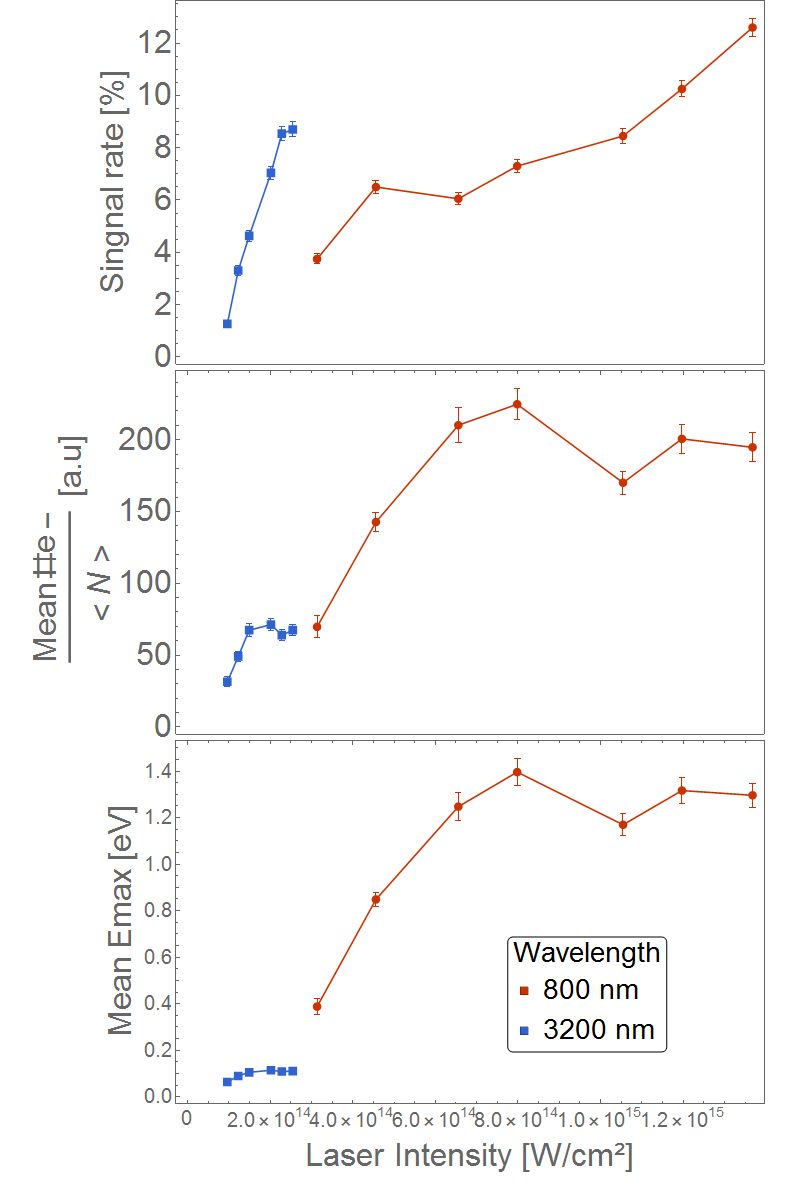
\includegraphics[width=1\textwidth]{../Images/results/Comparison_energyDistribution/Comp_Laser intensity.png} 
\end{subfigure} 
\begin{subfigure}[l]{0.48\textwidth}
\caption{Pulse dependence on Ne and He cluster in MIR laser fields}
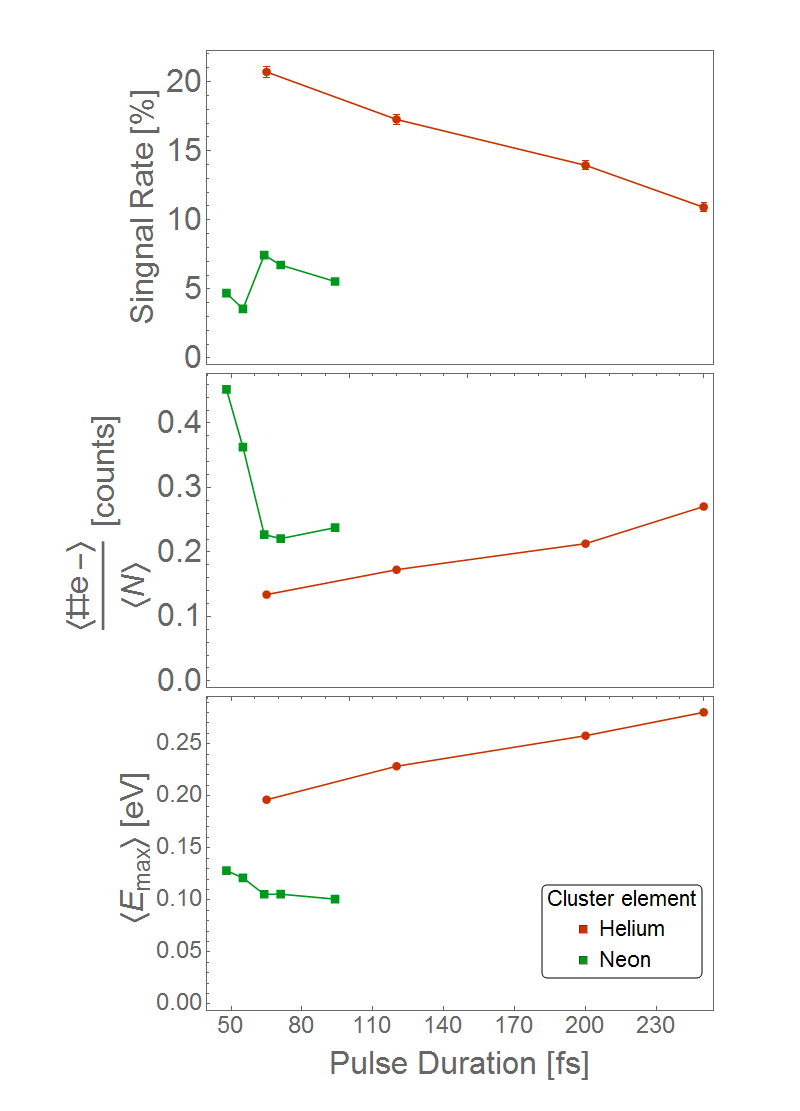
\includegraphics[width=1\textwidth]{../Images/results/Comparison_energyDistribution/Comp_pulseduration.png} 
\end{subfigure} 

\hfill
\caption[Laser parameter comparison]{Comparison of the pulse duration and laser intensity. On the right, the pulse duration dependency for the signal rate and mean values of He and Ne clusters. On the left, the laser intensity dependence for He cluster in NIR at 800 nm wavelength and MIR at 3200 nm wavelength.  The mean number of electron is normalized to the cluster size in both cases. }
\label{fig:lasercompar}
\end{figure}

Fig \ref{fig:lasercompar} shows the comparison for the experiments with different laser intensity and pulse duration. On the left we show the signal rates and mean values for the different laser intensities using He clusters interacting with the MIR and NIR laser. On one hand, there exist a linear dependence where the intensity increase the signal rate drastically, with both lines (blues and red) having a zero signal close to 8$\cdot$10$^{13}$ W/cm$^{2}$. As expected, there exist a minimum beam intensity to achieve plasma formation because the main energy transfer from the photons to the clusters is done via ionized dopant electrons that initiate the electronic cascade and forms the coulomb explosion. If the initial energy is not enough to ionize the dopant, none electrons will interact with the laser field and the plasma will not be create. On contrast, the signal rate in the MIR can be comparable to the NIR even at lower intensities, for example, He rate for the blue line at 2$\cdot$10$^{14}$ W/cm$^{2}$ is the same as the point at 8$\cdot$10$^{14}$ W/cm$^{2}$ in the blue curve. It also can be related to the doping level and the slightly size difference in each easement but both lines have a parallel behaviour that confirm our assumption 

On the other hand, despite the normalization at the cluster size, is clear that the NIR field produce more electrons at higher energies, reaching energies one order of magnitude higher than the MIR.  This could be interpreted that the 800 nm wavelength range in the plasma resonance and the cluster is ionized completed, even for the biggest droplets, as shown in the plateau for intensities upper than 1$\cdot$10$^{15}$ W/cm$^{2}$. In contrast, assuming a complete ionization and that the detector can reach almost all electrons coming out of the explosion, in the mean number of electrons the blued curve does not have such high values as the red, what could indicate that the plasma formation in MIR laser fields is incomplete or partial. 

Fig \ref{fig:lasercompar} b. shows the pulse duration dependence of big He and Ne cluster in the MIR laser. Although in Ne a vast part of the pulse measurement is missing, we still see some relation in the points around 60 to 100 fs. On top, the red signal rate presents an expected decrease in accordance to the laser intensity plot, the longer pulses have lower intensity, in consequence the signal rate goes down. Same happens for the blue curve, that in the 60 to 100 fs  range where it behaves parallel to the He line.
In contrast, a surprising result is shown in the mean values contrasting to the intensity dependence results. It shows that at longer pulses higher energies and electron numbers are achieve, in other words, it enhance the plasma formation for bigger droplets. Although, it is a non-intuitive results, it can be explained if we take into account that for longer pulses we have more cycles in the pulse. In consequence, even the initial ionization probability is lower for the first cycles, the electrons created on them will have more time to interact with the laser field, acquiring energy and boosting the electronic cascade to end in the coulomb explosion.

\section{Cluster Size Dependence}

As shown in fig \ref{fig:elementall} the droplet size plays an important role in the nanoplasma explosion. All clusters have a commune linear behaviour linked to the cluster size, the bigger the cluster more signal can be found.  On one hand, Ne cluster shows a more stiff tendency, its signal rates goes from 4 to 12$\%$  in small droplets compared to the He$_{NIR}$ at the smallest size does not goes up the 3$\%$. Moreover, either He$_{MIR}$ and He$_{NIR}$ have a continues growth for cluster around a few hundreds of thousands. In contrast at the biggest He$_{MIR}$ cluster shows a depletion of the signal, suggesting that exist a maximal cluster size where that MIR laser is not efficient any more, contrary to the NIR where at the same size, presents a enhance of its efficiency and for huge clusters reach a maxima according to the data. 

\begin{figure}[h!]
\caption[Cluster size comparison]{ Cluster size dependence of He and Ne cluster in MIR laser fields (yellow and blue), and He cluster in NIR laser (Red)the mean values are in logarithmic scales and the signal rate in linear scale.}
\centering
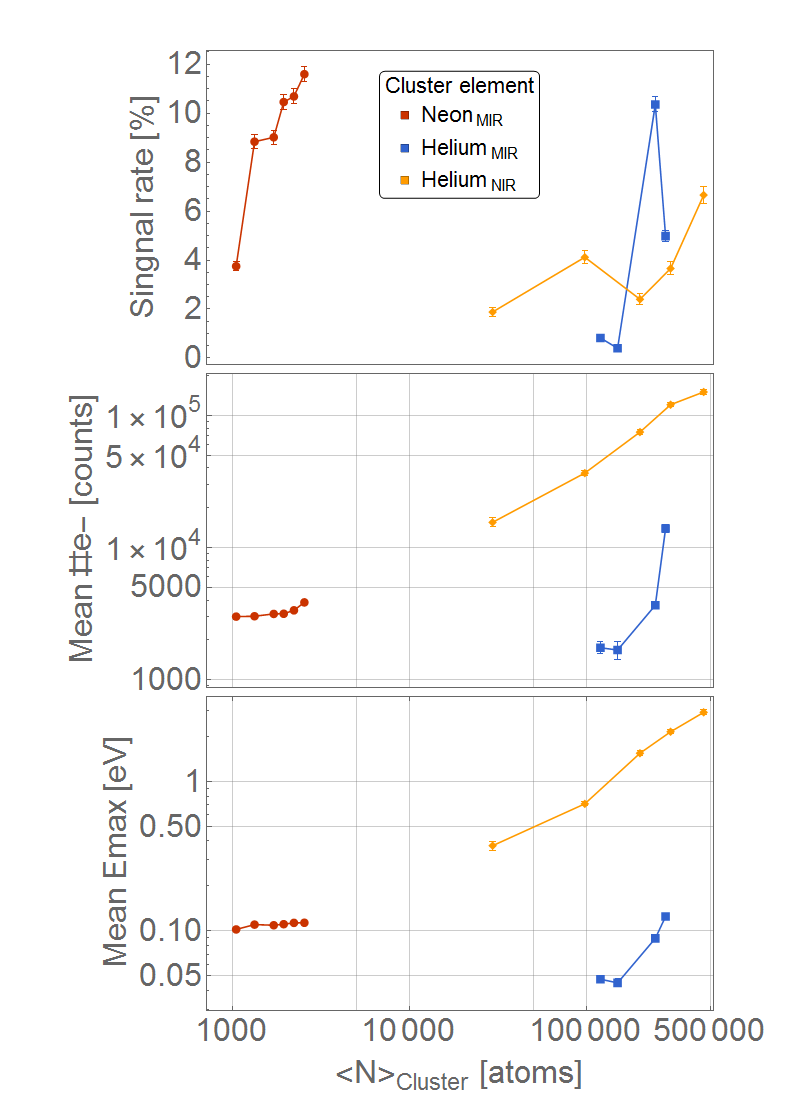
\includegraphics[width=0.6\textwidth]{../Images/results/Comparison_energyDistribution/Comp_clusterSize.png}
\label{fig:elementall}
\end{figure}

On the other hand, the mean values show a similar behaviour in the MIR independent of the cluster element, lines blue and red, have a similar values, having an initial constant trend and the bigger sizes have higher counts, yet in contrast the mean number of electrons  for the smallest droplets reach counts 2 order of magnitude lower. Same happens in the mean energy where the bigger droplets show higher energies, and all lines shows a similar trend. 
The reason for this tendency is not clear, but if we assume the interaction dopant-cluster, small cluster could have a high probability of losing the ionized electrons in the beginning of the pulse, so the ignition process is less efficient. However, for the bigger clusters, the ionized electron have more atoms to interact, so the losses reduces and in consequence the bigger clusters can be more efficient to create the nanoplasma. The reason for this tendency is not clear, but if we assume the interaction dopant-cluster, small cluster could have a high probability of losing the ionized electrons in the beginning of the pulse, so the ignition process is less efficient, while for the bigger clusters, the ionized electron have more atoms to interact, so the losses are less, and in consequence the bigger clusters are more efficient to create the nanoplasma.




\section{Doping Dependence}

Fig \ref{fig:dopcompari} shows an overview of all the mean values and signal rate for the He droplets with Ar, Xe and water, and Ne doped with Xe at different doping levels. On top the signal rate shows for He$_{2.5\cdot 10^{5}}$ similar values for low and high dopant. In contrast for the Ne$_{5000}$ at extreme low levels the signal rate goes to zero.  This lack of dynamics is an expected result, as explained, the MIR laser field does not have enough energy to ionize directly the He or Ne, so a dopant with a lower IP is needed in order to start the process. Once the process is started and the electronic cloud is formed, the extra  electrons given via the dopant ionization does not change the final result. The green line, Ne-Xe, is the only graph that have important changes. It suggests that the difference on cluster size between the Ne$_{5000}$ and He$_{2.5\cdot 10{5}}$ affect the cross section to get dopants and in consequence a minimum cluster size-doping preassure relation need to be achieve to effectively pickup Xe and so the plasma formation can start. This results shows that the doping can increase the efficiency to ignite the nanoplasma, and at large doping level the mean value of electrons decrease, meaning that we are igniting small droplets. In short, is more efficient to ignite bigger droplets than small ones, because according to the data, the small ones need a larger amount of doping to be ignited while the large cluster just need a few atoms.

\begin{figure}[hbtp]
\caption[Doping level comparison]{doping level dependence of He and Ne cluster in MIR laser fields doped with water, argon, and xenon in MIR fields.}
\centering
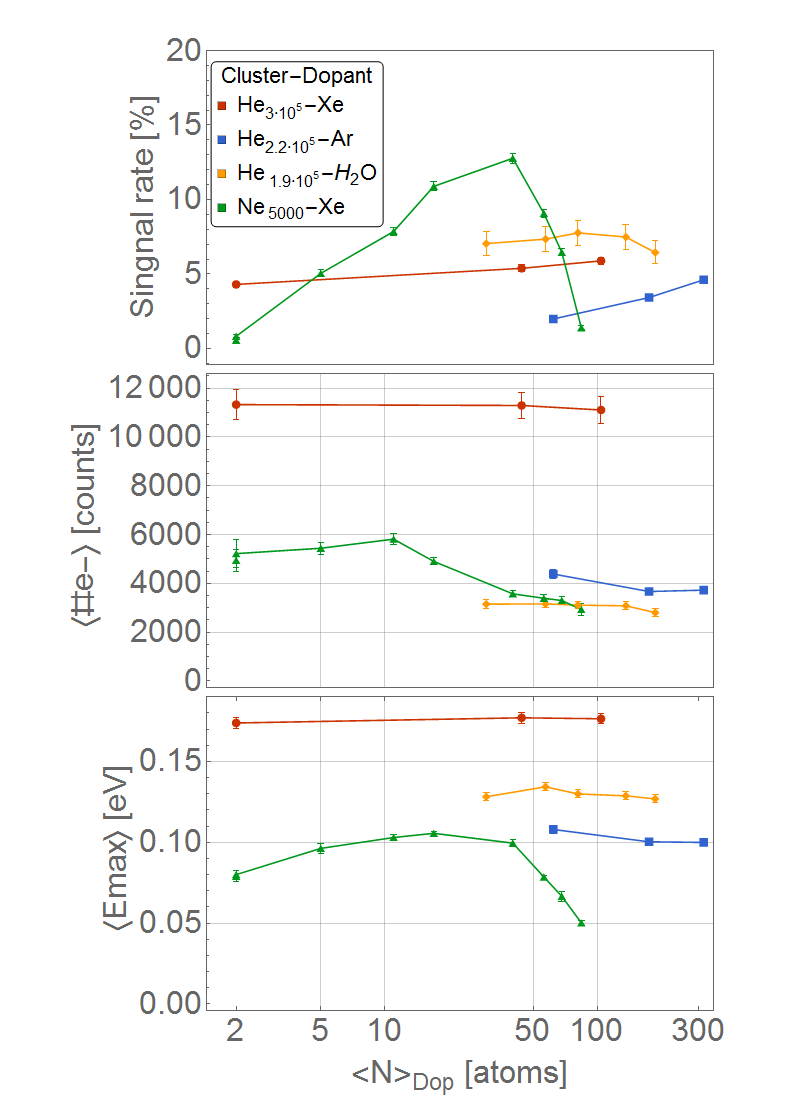
\includegraphics[width=0.6\textwidth]{../Images/results/Comparison_energyDistribution/Comp_AllDoping.png}
\label{fig:dopcompari}
\end{figure}

The mean values also shows a similar dynamics with steady He clusters independent on the dopant or the dopant level for He, while the Ne cluster present a constant grow for low doping levels showing a plateau around 50 atoms and a depletion for higher doping. It’s clear that, for the Ne line, the increase of dopants leads to an increase on the plasma formation, yet in case the dopant is to large, can be totally destroyed due the evaporation and cluster shrinkage, similar to the reports in other experiments \cite. 

Fig \ref{fig:XEcasig}, \ref{fig:XEcaelect} and \ref{fig:Xecaenerg}, shows the signal rate and mean values interpolation for the combination of Xe and Ca in He droplets in the MIR laser. The dashed color line are cuts at a constant dopant numbers, Xe+Ca at $40,50,65,85,100,120$ and $150$ atoms. The lines were choose in order that it lays between 3 data points, so the interpolation is accurate enough. On the right of each figure the cuts are plotted depending on the Xe atoms. It means that the right side of each line represent the doping with the maximum Xe atoms at the Xe+Ca constant, once we go from right to left, we replace each Xe atom for one Ca atom until all Xe atom are replaced. Each line have a maximum of 40 points, because it was the max Ca doping measured with enough statistics. 

\begin{figure}[h!]
\hfill
\begin{subfigure}[l]{0.48\textwidth}
\caption{MIR and Nir intensity dependence on He clusters}
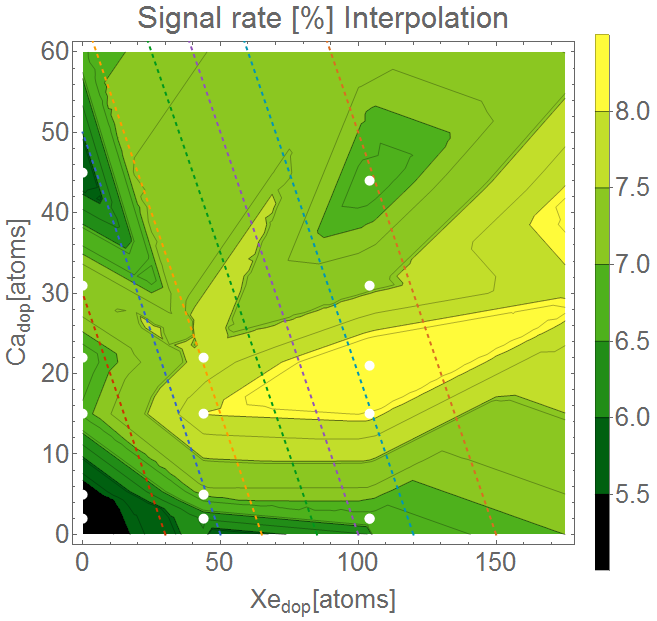
\includegraphics[width=1\textwidth]{../Images/results/MIR_He_XeCaDop/interpolationSignalRate.png} 
\end{subfigure} 
\begin{subfigure}[l]{0.48\textwidth}
\caption{Pulse dependence on Ne and He cluster}
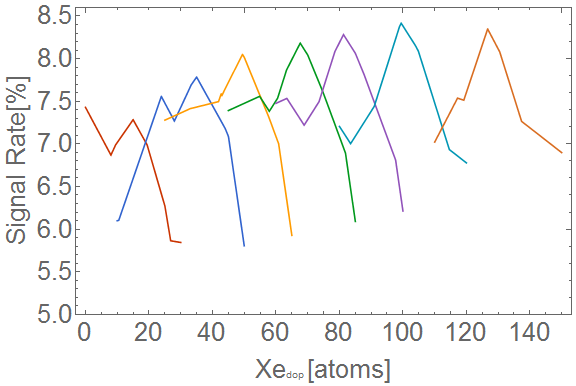
\includegraphics[width=1\textwidth]{../Images/results/MIR_He_XeCaDop/interpolationSignalRatelines.png} 
\end{subfigure} 
\hfill
\caption[Xe-Ca interpolation signal rate]{On the left, signal rate interpolation for He cluster doped with Xe and Ca at different doping levels.The white points correspond to the actual measurements and the dashed line the cuts at constant number of dopant atoms. On the right, the cuts for at a constant dopant numbers, Xe+Ca at $40,50,65,85,100,120$ and $150$ atoms for the corresponding color lines.}
\label{fig:XEcasig}
\end{figure}

An important result can de derive from Fig \ref{fig:XEcasig}, as shown in the cut lines at constant total doping, we found a increment in the signal as the Ca doping replace the Xe. In all line, from right to left, the signal rate goes up when a few atoms of Ca are added despite the amount of Xe. It demonstrate a better efficiency in the doping for Xe-Ca combination compared to only Xe or only Ca. This tendency can be spot not just on the big peak in the interpolation between 70 to 120 Xe atoms and 15 to 25 Ca atoms, but also in each of the cuts, where the lines clearly display a peak, the signal rate increase faster for these extra Ca atoms added. Once a saturation maxima is reach, the extra Ca atoms added makes the signal rate again decrees but in a slower way in most of the cases. 

\begin{figure}[h!]
\hfill
\begin{subfigure}[l]{0.48\textwidth}
\caption{MIR and Nir intensity dependence on He clusters}
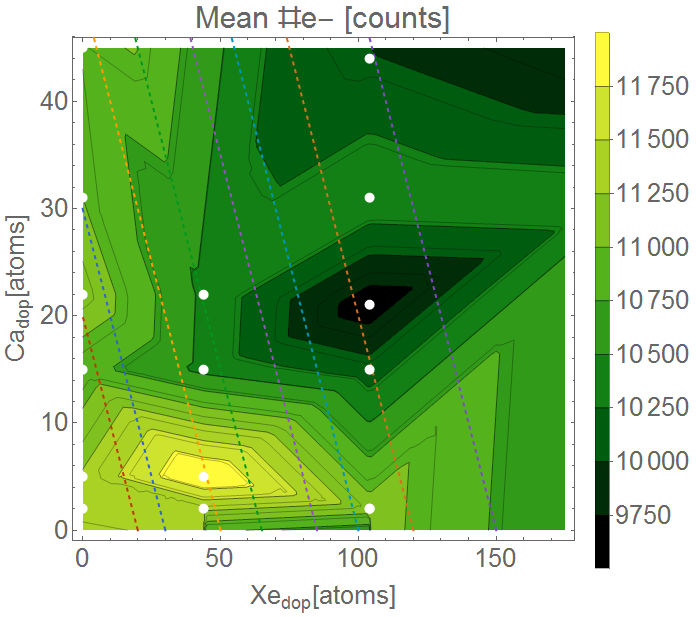
\includegraphics[width=1\textwidth]{../Images/results/MIR_He_XeCaDop/interpolationElectr.png} 
\end{subfigure} 
\begin{subfigure}[l]{0.48\textwidth}
\caption{Pulse dependence on Ne and He cluster}
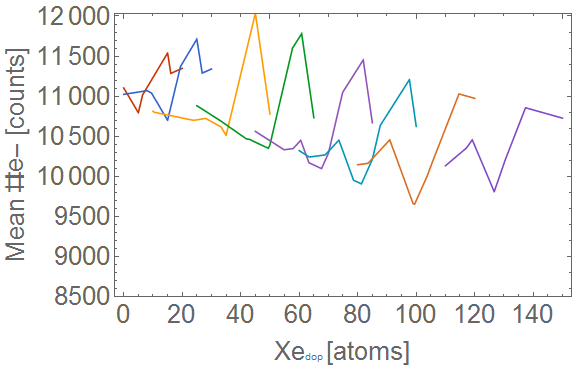
\includegraphics[width=1\textwidth]{../Images/results/MIR_He_XeCaDop/interpolationEleclines.png} 
\end{subfigure} 

\hfill
\caption[Xe-Ca interpolation num electrons]{ On left, the mean number of electrons interpolation for He cluster doped with Xe and Ca at different doping levels. On the right, the cuts for at a constant dopant numbers, Xe+Ca at $40,50,65,85,100,120$ and $150$ atoms for the corresponding color lines.   }
\label{fig:XEcaelect}
\end{figure}

Fig \ref{fig:XEcaelect} show one clear peak at low doping where the maximum  number of electrons appears, then for higher doping the counts starts to decreases and even a small depletion is shown in the range of Xe=100 Ca=20 atoms. On the right, the cut at constant dopant is show, the color from left to right represent the same cut done in the corresponding interpolation, and it’s necessary to read it at the same way. Where the right side of each line represents just Xe doping and each number to the left mean replacing one Xe atom for one Ca atom. As show, the exist also a recurrent peak efficiency in the nanoplasma ignition, meaning that at this peak the larger cluster are ionized, similar as shown on the Pulse duration scan.


\begin{figure}[h!]
\hfill
\begin{subfigure}[l]{0.48\textwidth}
\caption{MIR and Nir intensity dependence on He clusters}
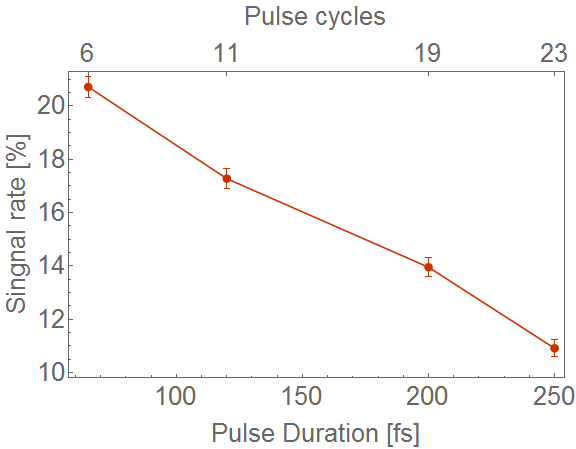
\includegraphics[width=1\textwidth]{../Images/results/MIR_He_XeCaDop/interpolationMax.png} 
\end{subfigure} 
\begin{subfigure}[l]{0.48\textwidth}
\caption{Pulse dependence on Ne and He cluster}
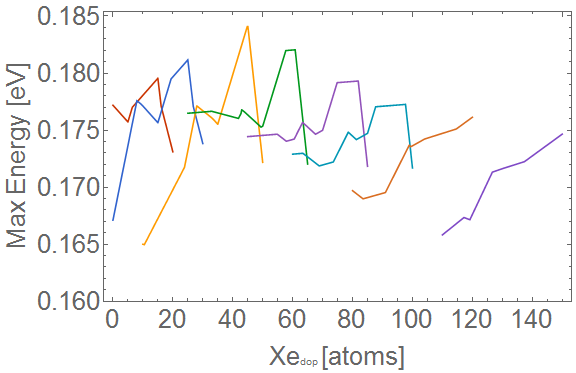
\includegraphics[width=1\textwidth]{../Images/results/MIR_He_XeCaDop/interpolationMaxlines.png} 
\end{subfigure} 

\hfill
\caption[Xe-Ca interpolation max energy]{On left, the mean max energy interpolation for He cluster doped with Xe and Ca at different doping levels. On the right, the cuts for at a constant dopant numbers, Xe+Ca at $40,50,65,85,100,120$ and $150$ atoms for the corresponding color lines. }
\label{fig:Xecaenerg}
\end{figure}

Equally important. In the E$_{max}$ interpolation, a clear peak is also shown at Xe= 50 and Ca=7 atom,  This can be found in interpolation cuts, where the highly doped lines have a more constant performance and no real change is shown, but once we get close to the optimum doping (Yellow line), the replacement of Xe atom for Ca atoms becomes drastic effective, with a peak  founded close to 0.2 eV.  This measurement can be compare directly to the water doping scan where we show that once the ignition of the cluster starts, adding more water atoms does not creates changes in the process. Here, Xe doping results in a similar behavior, the points with just Xe atoms (Right edge of each colored line) have a relative constant mean energy, but once we introduce the Ca, dynamics start to appears, given a peak close to the Mean electrons interpolation. For the heavily doped clusters, on the blue, orange and purple cuts in the right, we see that the peaks are not present any more due the cluster destruction when to many atoms are added.



\section{Electron-Energy Distribution}

Once the number of electron and max energy was extracted from each VMI picture, an energy distribution depending on the electrons detected can be plot to fitted to the uniform charge spherical model explained in chapter 1. The next figures will display the binned correlation for the max kinetic energy and number of electrons with their correspondent fit based on $E_{max}=B\cdot n^{2/3}$ Eq. 1.30, where $n$ is the number of electrons  and $B$ is the B-factor related to the electron density in the electronic cloud. The error bars are the standard derivation for the binned section and in case there is just one point in the binned region the error was assigned to the resolution of the experiment.

Fig \ref{fig:caxeinter} presents the data for He droplets in NIR laser fields for the cluster size dependence and the laser intensity measurements. Fig a. shows the binned energy distribution for the different droplets sizes. The red and purple line is a fit based on Eq. 1.30 where B is the B-Factor and $n$ is the number of electrons, the $2/3$ factor is fix to the fitting. The red and purple line correspond to the biggest and smaller droplets respectively, and all other fit lines showed the same tendency fit quite well to the data points. For the B-factor at Ne$_{4.6\cdot10^{5}}$ the corresponding electronic cloud density is around $\rho =2.2 [1/\mu m^{3}]$, what leads to an electronic cloud radius of  4.3 $\mu$m.
In Fig b. the same process is done for each of the data sets at different laser intensities. All fits have the same tendency regardless the laser intensities, changing slightly on the B-factor. This in an important outcome meaning that the data fits quite well to our simple spherical electronic cloud model. As the B-factor is directly related to the density of the electronic cloud using Eq. 1.3 is possible to delimit the radii of the electronic sphere. In other words, according to this model, if we know the total number of electrons it’s possible to calculate the maximal energy that we can detect. For the B-factor at 1.4$\cdot10^15$ W/cm$^{2}$ the corresponding electronic cloud density is around $\rho =0.02 [1/\mu m^{3}]$, what leads to an electronic cloud radius of  136 $\mu$m. The Inset on the top-left cornet shows the electron density for each of the laser intensities and cluster sizes, showing a strong dependence quit the cluster size a s expected but a similarity with the signal rate intensity dependence with a plateau in the higher laser intensities.


 \begin{figure}[h!]
\centering
\begin{subfigure}[t]{0.65\textwidth}
\caption{He cluster size dependence energy distribution in NIR laser pulses}
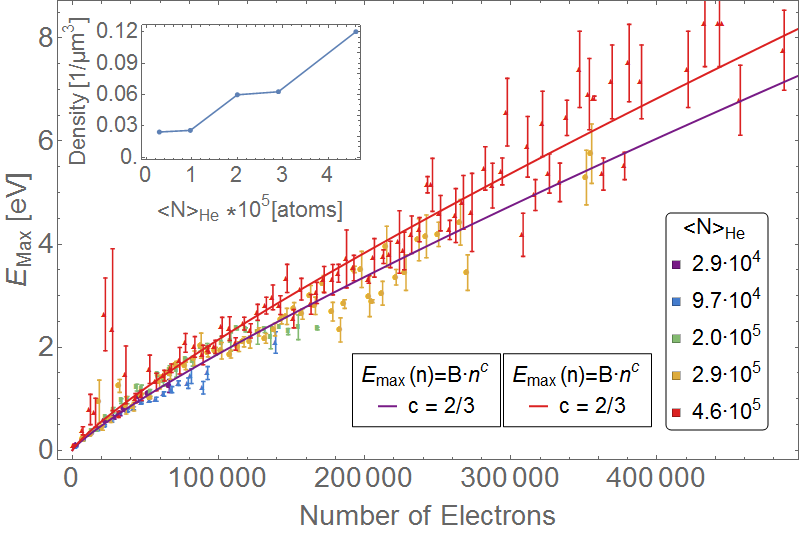
\includegraphics[width=1\textwidth]{../Images/results/NI_He_Dropletsize/vinned.png} 
\end{subfigure} 
\hfill

\centering
\begin{subfigure}[t]{0.65\textwidth}
\caption{Helaser intensity Dependence Energy distribution in NIR laser pulses}
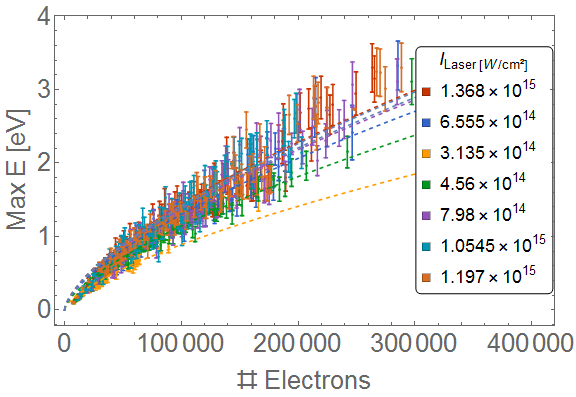
\includegraphics[width=1\textwidth]{../Images/results/NIR_He_intensityscan/binned.png} 
\end{subfigure} 
\hfill
\caption[Energy-Number of electrons relation. NIR Helium Droplets]{Energy distribution related to the number of electron for He clusters in NIR laser fields at different Cluster size fig a. and laser intensity Fig b.}
\label{fig:NIRcaxeinter}
\end{figure}


Fig \ref{fig:Heenrgd} presents the data for He droplets in MIR laser fields for the cluster size dependence and the Pulse Duration measurements. Fig a. presents the binned maximal kinetic energy distribution for different droplet size, the color points shows the different cluster sizes with the standard dispersion as error bars. The continue lines are fit lines with $c$ exponent fixed to $2/3$. It is clear that the continue lines deviates from the data, meaning that the spherical model cannot be applied for these measurements. Moreover, the dashed line is a fit based on the same equation but with the exponent $c$ free. As seen, this lines have a better agreements with the data, even though the analytical model cannot be applied in this case, there exist a clear correlation of the energy and number of electrons that a refinement of the model could solve in a future. This new exponent is persistent in all the fit for the MIR experiments in helium.  Fig B show another example where the spherical model (continues lines) fails and a better fit with the $c$ match the data (dash line)

There is no theoretical background that can predict this behaviour, one of the possible explanation, taking into account that the exponent is closely linked to the geometry of the cloud, is that the big droplets are not perfectly spherical, for example, because He is liquid, the droplets could turn in an ellipsoidal shapes. . A second reason can be because of the partial coulomb explosion described in the previous section. As describe, not all the cluster is generating a plasma and just part of it generates a nanoplasma, so the final electronic cloud will present abnormalities making its density and shape non uniform. Although our analytical model cannot describe precisely the energy distribution it is clear that the number of electron and max energy have a close relation and even the model does not fit, it can be possible to introduce some correction in the future to have a better model

 \begin{figure}[h!]
\hfill
\begin{subfigure}[l]{0.48\textwidth}
\caption{He cluster size dependence energy distribution in MIR laser pulses}
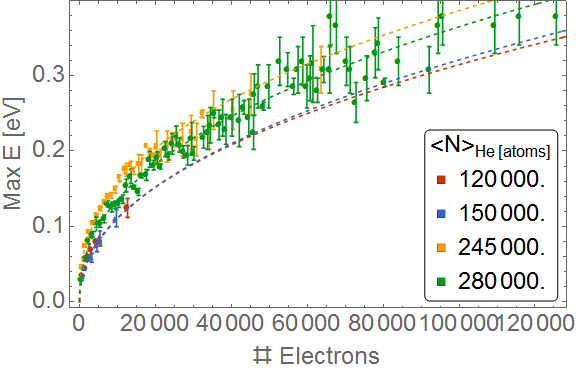
\includegraphics[width=1\textwidth]{../Images/results/Mir_He_Dropletsize/binned.png} 
\end{subfigure} 
\begin{subfigure}[l]{0.48\textwidth}
\caption{He pulse duration Dependence Energy distribution in MIR laser pulses}
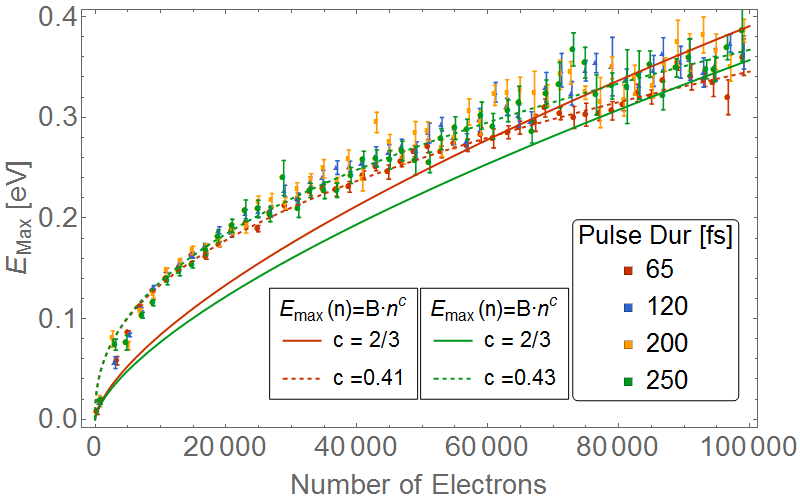
\includegraphics[width=1\textwidth]{../Images/results/MIR_He_pulsescan/raw/binned.png} 
\end{subfigure} 
\hfill
\caption[Energy-Number of electrons relation. MIR helium droplets]{Energy distribution related to the number of electron for He clusters in MIR laser fields at different Fig. a. and cluster sizes and pulse duration Fig. b.}
\label{fig:Heenrgd}
\end{figure}

Fig \ref{fig:Neenrgd} presents the data for Ne droplets in MIR laser fields for the cluster size dependence and the Xe dependence measurements, with $c$ and $B$ factor set free. In Fig a. The fit function are done for the shorts pulse with the c exponent at $2/3$ and as a free parameter. Once again the model does not fit but a clear energy distribution is present independent for the pulse duration. The dashed line follows $B=0.03$ and $c=0.23$ and is shared for the other data sets. 
Figure b. shows the Energy distribution with a similar trend, the data point and signal presents the same energy distribution as shown in the pulse scan. The fit function was done in the same way. The model fit shows and proximate better agreement to the first data point at lower energies but diverge rapidly to the bigger ones. The dash fit on the contrary show that the energy distribution follows a similar trend independent to the cluster size, but our spherical model cannot be applied.

 \begin{figure}[h!]
\hfill
\begin{subfigure}[l]{0.48\textwidth}
\caption{Ne Pulse length Dependence Energy distribution}
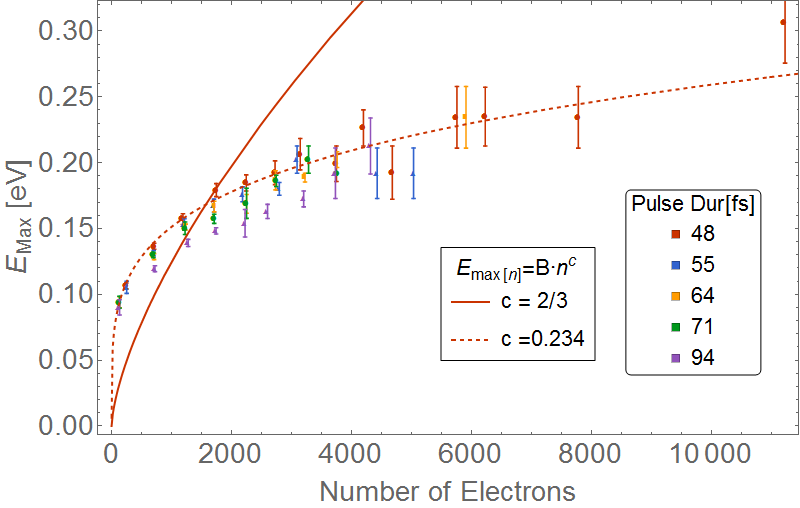
\includegraphics[width=1\textwidth]{../Images/results/MIR_Ne_pulseduration/binned2.png} 
\end{subfigure} 
\begin{subfigure}[l]{0.48\textwidth}
\caption{Ne Cluster size Dependence Energy distribution}
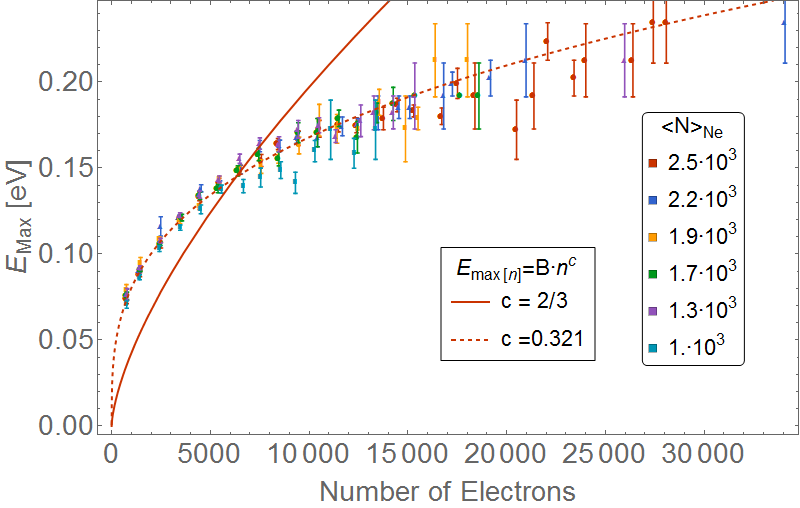
\includegraphics[width=1\textwidth]{../Images/results/MIR_Ne_DropletSize/binned.png} 
\end{subfigure} 
\hfill
\caption[Energy-Number of electrons relation. Neon Droplets]{Energy distribution related to the number of electron for Ne clusters in MIR laser fields at different pulse duration fig a. and cluster sizes Fig b.}
\label{fig:Neenrgd}
\end{figure}

